\documentclass[book]{jlreq}
\usepackage[bookmarks=true,bookmarksnumbered=true,
pdftitle={システム設計面接対策},
pdfauthor={中村 遼太郎},
pdfkeywords={System Design; Interview},
pdflang=ja-JP]{hyperref}
\usepackage{hyperref}
\usepackage{tikz}
\usepackage{graphicx}
\usepackage{main}
\NewPageStyle{system}{
  nombre_position=bottom-right,
  running_head_position=top-right,
  mark_format={_chapter={\thechapter 章 #1},_section={\thesection #1}},
  odd_running_head=_chapter,
  even_running_head=_section
}
\pagestyle{system}
\addbibresource{main.bib}
% Prevent the URLs the in bibliography section from overflow.
% https://ctan.math.illinois.edu/macros/latex/contrib/biblatex/doc/biblatex.pdf
% \setcounter{biburlnumpenalty}{100}
% \setcounter{biburlucpenalty}{100}
\setcounter{biburllcpenalty}{100}

\begin{document}
\title{システム設計}
\author{中村 遼太郎}
\date{\today}
\maketitle
\tableofcontents
\part{基本}
\begin{chapter-bib}{面接}
  \section{方針}
  システム全体のアーキテクチャを問われるときは、Propose a Design, Talk about trade-offs, Discuss design choices, Limitationsの4部構成で話す\cite{lc-high}。
  \section{マイクロサービス}
  課題はモノリスで設計するには複雑すぎるので、マイクロサービスの設計を提案する\cite{lc-aa}。
  \subsection{設問}
  \begin{exercise}
  \item モノリスと比べたときのマイクロサービスの利点と欠点をのべよ。\label{exe:monolith-micro}  
  \end{exercise}
  \subsection{解説}
  \subsubsection{\ref{exe:monolith-micro}}
  たとえば、複数の技術を適材適所に使えるが、プロセス内の通信がネットワーク越しのAPI呼び出しになる分のレイテンシーが発生する\cite{lc-aa}。
\end{chapter-bib}
\begin{chapter-bib}{指標}
  \section{レイテンシ}
  レイテンシはリクエストが処理を待っている時間である\cite{sdi}。
  レイテンシの許容範囲内でスループットが最大であることが望ましい\cite{sasp}。
  この目標は、スループットとレイテインシにあるトレードオフを示唆している。
  たとえば、バッファリングをもちいると、スループットを改善できるが、バッファ内で待機するデータのレイテンシは悪化する。
\end{chapter-bib}
\begin{chapter-bib}{メッセージング}
  \section{メッセージングサービス}
  AMQP (Advanced Message Queuing Protocol) はブローカーを介したメッセージングプロトコルの標準的な仕様であり、RabbitMQによって実装されている\cite{rabbitmq-amqp}。

  \section{Queue} 
  複数のサービスへ同期的に通信するトランザクションは、通信を非同期にすれば応答の待機時間を短くできる。
  しかし、対向サービスに障害があれば非同期通信が失敗しても、トランザクションは別のサービスにリクエストを送る。
  サービスをキューを介して通信させることで、対向サービスと一時的につながらない間でも、キューにメッセージを蓄積でき、メッセージの消失を防ぐことができる\cite{lc-isc}。
  
  また、メッセージのスパイクが起きてもブローカーがバッファとなり、負荷を平準化できる。

  ConsumerからProducerにキューを介してメッセージを送ることがある\cite{microsoft-messaging}。
  RabbitMQの場合、メッセージのヘッダにある\texttt{reply-to}にキューを指定し、Producerが処理結果を指定されたキューに送ることで、ProducerとConsumer間で双方向の通信ができる\cite{rabbitmq-direct-reply-to}。
  \subsection{設問}
  \begin{exercise}
  \item 2つのサービスが直接ではなくキューを介して非同期通信する利点をのべよ。また、利点を満足するためのキューへの要件は何か。\label{exe:async-queue}
  \item 主要なメッセージキューのミドルウェアを挙げ、向き、不向きを比較せよ。\label{exe:queue-compare}
  \end{exercise}
  \subsection{解説}
  \subsubsection*{\ref{exe:async-queue}}
  対向システムの障害時のリクエストをキューに一時的に保存できるため、失敗するリクエストを減らすことができる\cite{lc-isc}。
  キューは、中継対象のシステムより、安定していなけばならない。
  キューでなくロードバランサでも負荷分散を実現できるので、キューの利点として負荷分散を先にあげるのはよくないだろうか。
  \subsubsection*{\ref{exe:queue-compare}}
  Kafka, RabbitMQ, ActiveMQがある\cite{lc-isc}。
\end{chapter-bib}
\begin{chapter-bib}{双方向通信}
  \section{双方向通信}
  ロングポーリングは、タイムアウトまでの時間を長くし、サーバからの応答を待つ。
  このとき、サーバーはクライアウントのタイムアウトを検知できない\cite{sdi}。
  サーバーからの通知が必要でクライアントからの通知がいらなければ、WebSocketではなくEvent Sourceを使えるか検討するとよいかもしれない。
  2022年8月におけるTwitterのタイムラインには、Event Sourceが使われている。

  WebSocketはステートフルであるため、WebSocketサーバーを水平スケールする場合、ドレインするサーバーのコネクションを移し、新たなコネクションが追加されないようにしなければならない\cite{sdi2}。
  \subsection{設問}
  \begin{exercise}
  \item ロングポーリングとWebSocketそれぞれの使いどころを述べよ。
  \item WebsocketとEvent Sourceの利点欠点を比較せよ。
  \end{exercise}
\end{chapter-bib}
\begin{chapter-bib}{Pub/Sub}
  \section{Redis}
  RedisにはPub/Subの機能もある\cite{redis-pubsub}。
  数GBのメモリがあれば、数百万のチャネルを作れる\cite{sdi2}。
  ドキュメントを読む限り、すべてのSubscriberにメッセージをブロードキャストし、Ackによる再処理はできない。

  Expireコマンドを使えばエントリーにTTLを設定できる\cite{redis-expire}。

\end{chapter-bib}
\begin{chapter-bib}{CQRS}
  CQRSはデータをコマンドとクエリの両方のモデルで永続化する\cite{microsoft-cqrs}。
  % CQRSでEvent Sourcingが必須なのは、コマンドの永続化層にデータを書き込むのとをクエリの永続化層への追加したデータの通知を、1つのトランザクションで行い整合性を保つ必要があるから\cite{j5ik2o-cqrs-event-sourcing}。
\end{chapter-bib}
\begin{chapter-bib}{データベース}
  \section{データベース}
  % NOSQLの代表例, document指向の使いどろこ、列指向のつかいどころを説明させる。
  ACIDのConsistency(一貫性)は、データに常に真でなければならない不変性があることである\cite{ddia}。
  
  属性が多いデータはドキュメント指向データベースが、クエリのパターンが少ないがデータ量が多いときは列指向データベースがよい\cite{lc-databases}。
  
  ドキュメント指向データベースの例にMongoDBやCouchbaseが、列指向データベースの例にCassandraやHBaseがある。
  \section{冗長化}
  データベースのインスタンスをアプリケーションから直接参照させず、ロードバランサを参照することが推奨されている\cite{cs75}。
  データベースのロードバランシングにもHAProxyが使える\cite{haproxyMySQL}。
  
  ロードバランサを使わずにMySQLでフェイルオーバーを実現したい場合、JDBCならば、JDBC URLに複数のホストを指定すればよい\cite{MySQLJDBC}。
  \section{データ構造}
  \subsection{SSTable}
  SSTableは、Biggtableで使われるキーバリュー形式かつ追記型のデータ構造であり、かつキーと値のペアをキー順にセグメントに格納する\cite{ddia}。
  各セグメントごとにキーはユニークである。
  HBaseはSSTableを利用した列指向のデータベースである\cite{ddia}。
\end{chapter-bib}
\begin{chapter-bib}{キャッシュ}
  \section{キャッシュの書き込み}
  キャッシュの書き込みパターンに、write-throughとwrite-backがある\cite{sasp}。
  Write-throughは、キャッシュ、ストレージの順にデータを書き込み、ストレージに書き終えるまで、新たな書き込みをブロックする。
  Write-backはキャッシュにデータを書き込んだ後、非同期にキャッシュからストレージにデータを書き込み、ストレージへの書き込みが完了する前にもデータを受理する。
  
  \section{CDN}
  \subsection{Consistent Hashing}
  キャッシュを複数のノードに分散して保存するとき、ハッシュ関数をキーに適用し、値が格納されたノードを特定できる。
  このとき、参加するノードが変われば、キャッシュされたデータを再配置しなければならない。
  コンシステントハッシュ法は、円環上のハッシュ値とノードを配置したとき、ハッシュ値から時計回りに出発し最初に出会うノードに値を格納する\cite{sdi}。
  このとき、ノードを追加、削除した場合に変更が起きた箇所付近の弧のノードだけをリバランスすればよく、再配置すべきデータ量を減らすことができる。
  ノードの数が少ないと、再配置した結果、ノードごとのデータ量が偏るおそれがある。
  ノードの数がおおいほど、偏りを防げるため、1つのノードに対応する複数の仮想的なノードを円環上に配置することで、偏りを抑止できる。
  
  Consistent Hasingは、CDNのようなインターネット規模のキャッシュシステムで使われるが、データベースのパーティショニングではうまくいかない\cite{DBLP:journals/corr/LampingV14}。
  \subsection{Varnish}
  ウェブアクセラレータはリバースプロキシやロードバランサの仕組みでウェブサイトを高速化するミドルウェアであり、VarnishはリバースプロキシとしてHTTPレスポンスをキャッシュする\cite{varnish,webaccel}。
  VarnishでプライベートなCDNを構築するときも使われる\cite{varnish-private-cdn}。
  \section{Cache Eviction}
  Cache evictionの方式にはTTL、FIFO, LFU, LRU, LFRUなどがある\cite{lc-cache}。
\end{chapter-bib}
\begin{chapter-bib}{分散ファイルシステム}
  CDNを使えば、Amazon S3などの分散ファイルシステムに配置したデータを高速に配信できる\cite{lc-databases}。
\end{chapter-bib}
\begin{chapter-bib}{Rate Limiting}
  \section{Leaky Bucket}
  蓄えられる未処理のリクエスト数と一定時間に処理できるリスエスト数の2つパラメータでリクエストを制御する\cite{sdi}。
  蓄えられている未処理のリクエストから一定時間内の固定数のリクエストを処理する。
  蓄えられるリクエスト数を越えてリクエストが届く場合リクエストを破棄する。
  パラメタ数が少なくチューニングが簡単だが、蓄えられるリクエスト数が一杯になるまでは、一定時間に処理できる分量以上のリクエストを受けつけてしまう。
  \section{Fixed Window}
  一定時間のウィンドウ内に処理するリクエスト数の上限を決め、それを越えるリクエストを破棄する。
  2つのウィンドウをまたいだ時刻にリクエストが多く到着する場合、ウィンドウサイズを越えたリクエスト数がウィンドウサイズと同じ時間内に処理されるおそれがある。
  \section{Sliding Window}
  一定時間のウィンドウをスライドさせ、Fixed windowのウィンドウをまたいだ場合に上限以上のリクエストが処理される問題をふせぐ。
  Fixed Windowよりも制御に多く計算リソースが必要である。
  \subsection{設問}
  \begin{exercise}
  \item リクエストの上限を制御するためのアルゴリズムをいくつか挙げ、その特徴をのべよ。
  \end{exercise}
\end{chapter-bib}
\begin{chapter-bib}{Web RTC}
  Web RTCはリアルタイム通信の標準規格である\cite{webrtc}。
  NATの後方にいるピアと接続するには、NATをバイパスしなければならない。
  Interactive Connectivity Establishment(ICE)は、直接接続できないピア間の通信を確立するためのフレームワークであり、STUN(Session Traversal Utilities for NAT)やTURN(Traversal Using Relays around NAT)プロトコルを提供するサーバを立て、ピアを接続する\cite{mdn-webrtc}。
  STUNサーバーは、ピアとの直接接続を妨害するルータの制限を特定する。
  例えば、ルータの制限がSymmetric NATであば、ルーターは過去に接続したことのあるピアからの接続しか受け入れない。
  この場合、ピアはTURNサーバにパケットを送信し、TURNサーバがパケットを相手に送信する。
  TURNサーバの負荷が大きいため、STUNサーバが他の通信手段を見つけたら、TURNはもちいられない。
\end{chapter-bib}
\begin{chapter-bib}{Back of envelope}
  Back of envelopeに使う要素を覚えておきたい。
  1日なので$24*60*60=86400$秒であるからおよそ$10^5$とみなす\cite{sdi2}。
\end{chapter-bib}

\begin{chapter-bib}{ロードバランサ}
  \section{DNSラウンドロビン}
  DNSラウンドロビンは、DNSに複数のAレコードを登録することによるラウンドロビン形式の負荷分散である。
  簡単だが、分散先のサーバーの活性や負荷状況に関係なく分散する欠点がある\cite{cs75}。
  \section{冗長化}
  ロードバランサも冗長化しなければ、ロードバランサ自体が単一点障害を生んでしまうおそれがある。
  冗長化するときは、ロードバランサーから別のロードバランサーにハートビートを送る\cite{cs75}。
\end{chapter-bib}
\part{Case Studies}
\chapter{temp}
\begin{section-bib}{Google Maps}
  System Design Interview 2とLeetCodeのどちらの模範回答もユーザーの位置を表示する機能と目的地までの案内の機能を提供するサービスが分かれている\cite{sdi2,lc-googlemaps}。
  図\ref{fig:sdi2-googlemaps}のActive UsersやPersonalization DBなどの一部のDBについては、使うべきDBの種類が解説\cite{sdi2}に記載されてない。
  Cassandraの削除は遅い\cite{cassandra-delete}ので、Active Usersなど一時的なデータの格納には向かないと思われる。 
  \begin{figure}
    \centering
    \includegraphics[keepaspectratio, scale=0.25]{build/googlemaps.eps} 
    \caption{System Design Interview 2の模範回答}
    \label{fig:sdi2-googlemaps}
  \end{figure}
  全ユーザのモバイルアプリケーションを開発者の指定したタイミイングで一斉にアップグレードすることはできないので、後方互換性を守りにくい機能はモバイルアプリケーションではなくバックエンドに置かねばならない\cite{sdi2}。
  
  \subsection{LeetCode}
  解答は、ユーザの位置を特定する機能とユーザに道案内を提示する機能に対して個別のアーキテクチャ図を提示する\cite{lc-googlemaps}。
  ユーザの位置情報からマップを更新する。
  Spark Streaming Serviceは、新しいストリーミングサービスに置き変わった\cite{spark-streaming}。
  以下の機能要件は、二点間を移動中に距離とETAを随時通知することであり、ユーザが明示的にリクエストを移動中に送るだけではない。
  Google Mapは地図をcanvas要素で描画する。
  \begin{quote}
    Find distance and ETA while travelling between 2 points.
  \end{quote}
  
  \subsubsection{User Location Information}
  \begin{description}[labelsep=10pt]
  \item[Websocket Handler] ゲートウェイの役割。スケールアウトする。
  \item[Websocket Manager] デバイスがどのWebsocket Handlerと通信しているかを記録する。
  \item[Location Service] ユーザの位置情報を管理する。
  \item[Map Update Service] 新しい道などの地理的な変化を通知する。
  \item[Traffic Update Service] 移動速度の変化を通知する。
  \item[Graph Processing Service] グラフを更新する。
  \end{description}
  \subsubsection{User Navigation Flow}
  \begin{description}[labelsep=10pt]
  \item[Area Search Service] 現在値を緯度経度に変換する。
  \item[Navigation Tracking Service] ユーザが移動中に道案内を通知する。
  \item[Maps Service] ユーザからの道案内のリクエストを受けつける。
  \item[Historical data service] 過去のETAを蓄積し、最新のETAを計算できないときに、代替としてETAを提供する。
  \item[Segments]
  \end{description}
  \subsubsection{自分の解答}
  \href{https://docs.google.com/drawings/d/1w_a6eJVLqFsHHtm0dchQxM1NNOsW16ENjF7n_MRv6OE/edit}{編集中}
  \begin{figure}[!ht]
    \centering
    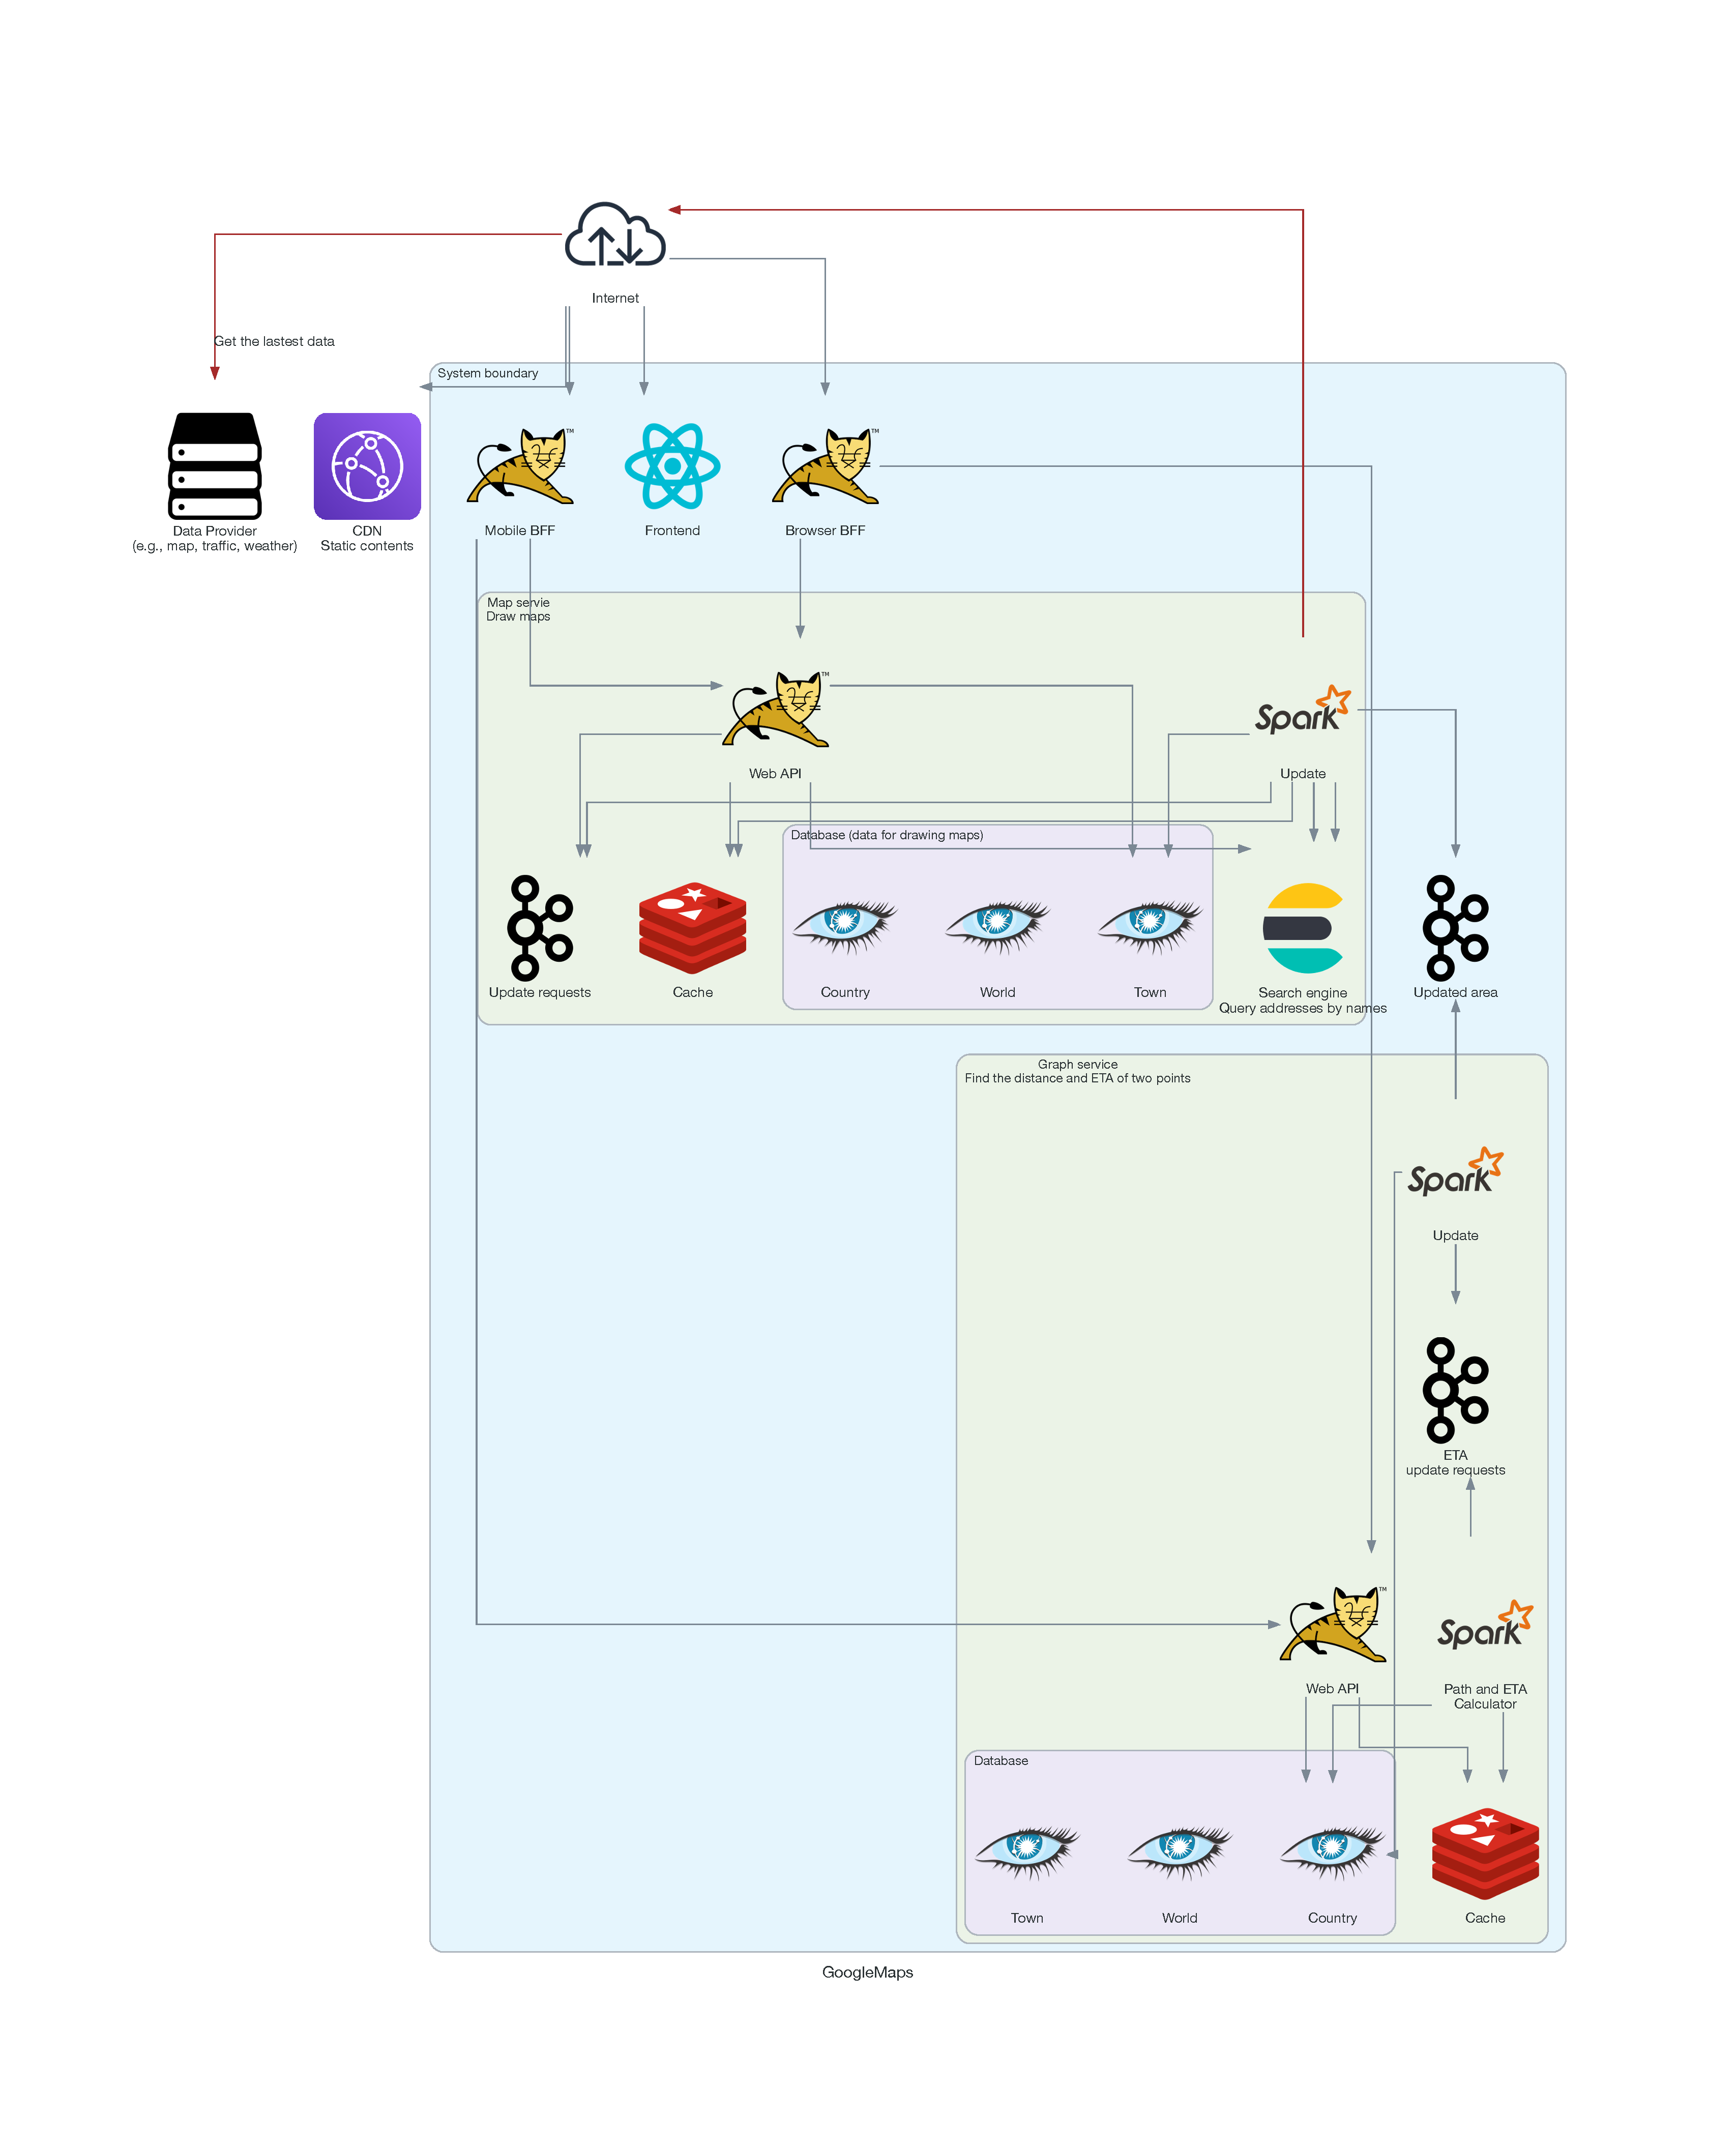
\includegraphics[keepaspectratio, scale=0.25]{build/googlemaps/leetcode.eps} 
    \caption{Googlemapsの答案}
    \label{fig:lc-googlemaps}
  \end{figure}
\end{section-bib}
\begin{chapter-bib}{Proximity Service}
地理情報に高速にアクセスする必要がある。
データの次元数がインデックスを使ったアクセスを高速化できる。
RDBMSのインデックスであるGeoHashは、地球を4分割し、4つに00, 01, 11, 10とコードを割り当てる。
さらに00の地域を4分割した地域に分割前の地域のコードをプレフィックスにして0000, 0001, 0010, 0011と再帰的に割り当てる。
この場合、プレフィックスが同じコードの地域は近隣であるが、逆は成り立たない\cite{sdi2}。

QuadtreeはGeoHashと同じく再帰的にデータの4分割を繰り返す\cite{quadtree}。
例えばお店の数などの条件をノードが満たさなければ、ノードを最大4つの子ノードまで分岐させる。

S2Geometry\cite{s2geometry}は空間充填曲線であるヒルベルト曲線を応用し、近い地域には距離の近い一次元のインデックスを割り当てる。

今回のシステムでは地理情報のデータサイズが小さいので、アプリケーションレイヤーにロジックが必要になるシャーディングよりも、リードレプリカでスケールするほうが望ましい。シャーディングは管理が複雑なので、リードレプリカで十分であれば、そちらのほうが望ましい。
\end{chapter-bib}
\begin{chapter-bib}{Nearby Friends}
  WebSocketの代わりにErlangをもちいてもいいとある\cite{sdi2}。
  \section{Back of envelope}
  \begin{itemize}
  \item ユーザ総数は10億人
  \item 同時アクセスユーザ数はユーザ総数の10\%である1億人いる。
  \item ユーザーは平均して400人の友人がいる。
  \item 各ユーザーは平均100人の友達の位置を情報を購読している。
  \item 位置を通知するRedisのチャンネルを1人が購読するごとに20バイトのメモリが必要になる。
  \item 30秒ごとにユーザを位置情報をサーバーに送る。
  \item ギガバイトクラスのネットワークにある1台のRedisサーバーは秒間10万件のイベントをPushできるとする。これは保守的な見積りである。
  \end{itemize}
\end{chapter-bib}
\begin{chapter-bib}{Distributed Message Queue}
  \section{要件}
  \begin{itemize}
  \item キューに格納できるメッセージサイズの上限はいくつか
  \item メッセージを再取得できるか
  \item 取り出せるメッセージの順序はFIFOか
  \item キューにあるメッセージの保存期間の長さは何か。
  \item メッセージの重複の性質は、exactly once, at-least once, at-most onceなどのいずれか。
  \item バイナリデータをメッセージで送れるか
  \end{itemize}
  キューに格納できるメッセージの量を増やすためにトピックをpartitionに分割し、複数のbrokerが個別のparititonのメッセージを配信する。
  SPOFを避けるために複数のbrokerにpartitionを複製する。複製されたpartitionには、leaderとfollowerの関係がある。
  Write Ahead Logでpartitonのメッセージを記録する。Write Ahead Logは追記とランダム読み込みのみ可能なファイルである\cite{sdi2}。
  partitionのWrite Ahead Logをセグメントに分割する。
  末尾のセグメントは読み込みと追記を、それ以外のセグメントは読み込みのみを可能とする。
  
  Consumerがメッセージをどこまで取得したかを記録しておく必要がある。
  BrokerがConsumerの状態を保存する\cite{sdi2}こともあれば、KafkaのようにConsumerが自分の状態を保存する\cite{Kreps2011KafkaA}こともある。
  Zookeeperやetcなどによるリーダー選出アルゴリズムでBrokerの中からリーダーを決め、Broker全体を管理させる。
  リーダーは、brokerを追加、削除するときに、paritionを再配置する。
  
  Producerは、leader paritionにメッセージを送信する。
  Consumerはどうやってメッセージが保存されているパーティションを特定するのか。

  Consumerグループごとに一台の調整役のBrokerがいて、このBrokerがComsumerにparitionを割りあてる。
  Consumerは調整役をグループ名から特定できる。
  Consumerがグループへの参加を調整役のにリクエストすると、調整役は既存のConsumerを含めてConsumerにparitionを割り当てなおす。

  at-most onceの場合、ProducerはBrokerからのACKを待たず、Consumerはメッセージを処理する前にcommitする。
  at-least onceの場合、ProducerはBrokerからのACKが返るまでメッセージを送り、Consumerはメッセージの処理の終了後にcommitする。
\end{chapter-bib}
\begin{chapter-bib}{Amazon System Design}
  \href{https://docs.google.com/drawings/d/156NaHO0stF_xJBGtAUzkLmhU2eIz2ZYGaySqlPKHCLY/edit}{編集中}。
  解答\cite{lc-amazon}の問題点と長所をいれて改修する。
  データの更新情報のフローがない。
  非同期結果整合性でよくとりこぼしがないほうがいいところはkafkaにしよう。
  \begin{figure}[ht]
    \centering
    \includegraphics[width=\textwidth,keepaspectratio]
    {build/amazon/leetcode.png}
    \caption{Amazonの答案}
    \label{fig:lc-amazon}
  \end{figure}
\end{chapter-bib}
\begin{chapter-bib}{Facebook System Design}
  \section{LeetCode}
  \subsection{答案}
  \href{https://docs.google.com/drawings/d/1Xe7tRV1plpmUM1GEbcm1Rr-Sl4nuBaOe9AlLlUXsHQw/edit}{編集中}。
  タイムラインに表示すべきPostのユーザを管理するために必要な抽象データ構造は、ユーザIDからユーザIDの集合を要素とするハッシュテーブルであるため、タイムラインの表示にグラフDBはいらない。
  BFFを使うとオーケストレーターパターン\cite{microsoft-choreography}になってしまうのだろうか。
  メッセージサービスを制御の反転につかえそう。
  タイムラインの要件が曖昧であれば、タイムラインの順序が厳密な時系列であるべきか聞いたほうがよさそう。
  Postはスパイクする可能性があり、また、高速に保存するため、処理の平準化のためにメッセージングサービスを間においた。
  TimelineとBFFはEventSourceで通信する。Timelineがstored postsを取得したら通知する。
  
  \begin{figure}[ht]
    \centering
    \includegraphics[width=\textwidth,keepaspectratio]
    {build/facebook/leetcode.png}
    \caption{Facebookの答案}
    \label{fig:lc-facebook}
  \end{figure}
  \subsubsection{Leetcodeの解答}
  Post Injestion Service\cite{lc-facebook}はPostの書き込みを、Post Serviceは読み込みを担当しているが、永続化層はコマンドとクエリに分かれておらず、CQRSではない\cite{microsoft-cqrs}。
  Kafkaは、ポーリングを避けてイベントをほかのサービスに通知するために使われているのだろうか。
  KafkaのConsumerが失敗した場合の処理を考慮していないのではないか。
  \subsection{設問}
  \begin{exercise}
  \item CDNにおいたファイルへのアクセスに認証をかける手段を実在のサービスをまじえて例示せよ。
  \item Kafkaのメッセージの順序は到着順か。
  \item Cassandraは集計関数があるか。たとえば、Likeの総数を誰がどのPostにLikeしたかを示すレコードから集計できるか。
  \end{exercise}
\end{chapter-bib}
\begin{chapter-bib}{Airbnb System Design}
  \section{LeetCode}
  文章ではなく動画で解説がなされてる\cite{lc-airbnb}。
  動画のある機能要件と非機能要件を列挙する。
  模範回答のアーキテクチャは他のLeetCodeの回答とおなじくKafkaを多用した非同期アーキテクチャだが、System Design Interviewはメッセージングサービスを使っていない\cite{sdi2}。
  LeetCodeの回答はKafkaを使った非同期アーキテクチャに偏向しているように思える。

  氏名やアドレスなどのユーザの予約以外の情報を保存する専用のサービスがない。予約していないユーザデータもBookingに保存するのだろうか。
  \begin{itemize}
  \item 機能要件
    \begin{itemize}
    \item Hotel
      \begin{itemize}
      \item Onboarding
      \item Updating
      \item Bookings
      \end{itemize}
    \item User
      \begin{itemize}
      \item Search
      \item Book
      \item Check Bookings
      \end{itemize}
    \end{itemize}
  \item 非機能要件
    \begin{itemize}
    \item Low latency
    \item High availability
    \item High consistency
    \item Scale
      \begin{itemize}
      \item 500K hotels
      \item 10M rooms
      \item 1000 rooms / hotel (max 7,500)
      \end{itemize}
    \end{itemize}
  \end{itemize}
  \subsection{答案}
  \href{https://docs.google.com/drawings/d/1oregVo4fx3HTBSgF3dMn4DQ3X_REdrHiq2u5p3FegcQ/edit}{編集中}
  \begin{figure}[ht]
    \centering
    \includegraphics[width=\textwidth,keepaspectratio]
    {build/airbnb/leetcode.png}
    \caption{Airbnbの答案}
    \label{fig:lc-airbnb}
  \end{figure}
\end{chapter-bib}
\section{Video Streaming Service System Design}
  \subsection{LeetCode}
  \subsubsection{模範回答}
  \begin{itemize}
  \item 機能要件
    \begin{itemize}
    \item Upload videos
    \item Users' homepage
    \item Search
    \item Play Videos
    \item Support all devices
    \end{itemize}
  \item 非機能要件
    \begin{itemize}
    \item Low latency
    \item High availability
    \end{itemize}
  \end{itemize}
  \href{https://leetcode.com/explore/learn/card/system-design/690/system-design-case-studies/4388/}{模範回答}には海賊版対策の機能がある。アップロードの終了を通知するサービスがある。
  CDNのリンクを特定するサービスがいる。
  \subsubsection{答案}
  \href{https://docs.google.com/drawings/d/1GL0j7JJm0ip7DnNsdWOHBbfoHmz5U1LwwcTsbRD7IZ4/edit}{答案}。  
  \begin{figure}[ht]
    \centering
    \includegraphics[width=\textwidth,keepaspectratio]
    {build/netflix/leetcode.png}
    \caption{答案}
    \label{fig:netflix-lc}
  \end{figure}

\section{Notification Service System Design}
  \subsection{LeetCode}
  \href{https://leetcode.com/explore/learn/card/system-design/690/system-design-case-studies/4389/}{模範回答}。
  送信先のユーザを登録するなどの通知用の外部サービスへの変更を適用する機能がない。
  \subsubsection{答案}
  \begin{figure}[ht]
    \centering
    \includegraphics[width=\textwidth,keepaspectratio]
    {build/notification/leetcode.png}
    \caption{Notification Sevice System Designの答案}
    \label{fig:notification-lc}
  \end{figure}  
\begin{chapter-bib}{Design a URL Shorter}
  \section{概要}
  LeetCodeとCracking the System Design Interview\cite{sdi}の解説における要所は、短いURLを重複なく発行するアルゴリズムにある。
  \subsection{LeetCode}
  \href{https://leetcode.com/explore/learn/card/system-design/690/system-design-case-studies/4390/}{問題文}。
  \href{https://docs.google.com/drawings/d/12tMudFwu-JWC6Hip34f5Js5eKX3KiAz1QffMaffhDb4/edit}{答案}。
  \subsection{Cracking the System Design Interview}
  重複検知にブルームフィルタ\cite{bloomfilter}か\href{https://en.wikipedia.org/wiki/Base62}{Base62}を使う。
  ブルームフィルタは、偽陽性を許容し、ハッシュ値の保持に必要な空間を抑えることで、空間効率を上げる\cite{bloomfilter}。
  ハッシュ空間には0からNまでのアドレスをもつNビットの空間をつかう。 要素のない初期状態では、すべてに0初期化される。 ある要素を空間に追加するときは、ハッシュコーディングで0からN-1までの値をとりえるd個の値を要素から計算し、そのd個のアドレスに1を格納する。 要素が空間に含まれるか確かめるときは、追加時と同様、d個のアドレスを求める。 そして、d個のアドレスにある全ての値が1であれば要素が存在し、それ以外は存在しないとみなす。
Base62は数字とアルファベットからなる62進数による数値の表現である\cite{base62}。
互いに素な定数$b$と$h$をつかった以下のrolling hash関数をつかえばハッシュ値を生成できる\cite{rollinghash}。
  \[ H = (c_1b^{m-1} + c_2 b^{m-2} + \dots + c_mb^0 ) mod h\]
\end{chapter-bib}
\begin{chapter-bib}{Twitter System Design}
  \section{LeetCode}
  \href{https://docs.google.com/drawings/d/1SU6qTfwFEy_aSr-Ik-FPNRJ2zWeNa6SuyRc64uyhPuo/edit}{答案}。
  \href{https://leetcode.com/explore/learn/card/system-design/690/system-design-case-studies/4391/}{模範回答}も\cite{ddia}もフォロワー数の多いユーザのツイートの配信と多くないユーザの配信処理を分けている。
  ユーザがタイムラインを参照する前に、タイムラインをキャッシュしておく。フォロー中のユーザがツイートしたら、フォローしているユーザの各タイムラインのキャッシュにツイートを追加する。ただし、ツイートしたユーザのフォロワー数が多いと追加する量が多くなるので、キャッシュには含めない。
  タイムラインのリクエスト時に、フォロワー数の多いユーザのツイートを取得する。
  \begin{figure}[ht]
    \centering
    \includegraphics[width=\textwidth,keepaspectratio]
    {build/twitter/leetcode.png}
    \caption{答案}
    \label{fig:twitter-lc}
  \end{figure}  
\end{chapter-bib}

\section{Uber System Design}
  \subsection{LeetCode}
  \href{https://docs.google.com/drawings/d/17wu9iCxfs3y7cy0ju6e3muZfvcxftr6B_zcXmRW_7qU/edit}{答案}。\href{https://leetcode.com/explore/learn/card/system-design/690/system-design-case-studies/4392/}{解答}。ドライバーと客が別のアプリケーションを使うことが前提。現在のタクシーの位置だけでなく、監査のためにこれまでの移動も記録したい。
  \begin{figure}[ht]
    \centering
    \includegraphics[width=\textwidth,keepaspectratio]
    {build/uber/leetcode.png}
    \caption{答案}
    \label{fig:uber-lc}
  \end{figure}    

\begin{chapter-bib}{WhatsApp System Design}
  \section{LeetCode}
  \href{https://docs.google.com/drawings/d/1CaZsUs1I5e0AHrzG1GERoX6WQeUtd3BQ0XrVHziaP1g/edit}{答案}。
  \href{https://leetcode.com/explore/learn/card/system-design/690/system-design-case-studies/4393/}{解答}。
  複数のWebSocket serverとそれらを束ねるWebSocket managerでユーザが使用中かを判定する。WebSocket server, managerの方式は以前の問題でも見た記憶がある。
  Whatsappのメッセージは相手に受信すると削除されるらしい。
  Cassandraの削除は処理性能を悪化させる\cite{cassandra-delete}。
  \begin{figure}[ht]
    \centering
    \includegraphics[width=\textwidth,keepaspectratio]
    {build/whatsapp/leetcode.png}
    \caption{答案}
    \label{fig:whatsapp-lc}
  \end{figure}
\end{chapter-bib}
\begin{chapter-bib}{Zoom System Design}
  \href{https://docs.google.com/drawings/d/1A7J7ts0KVsf5UxgRo8Geuezmy9dpJSeCJEHUTaqzB88/edit}{答案}。
  \href{https://leetcode.com/explore/learn/card/system-design/690/system-design-case-studies/4394/}{解答}。
 トランスコードは、デジタル映像をアナログ信号にデコードしないでデジタル信号のまま再エンコードすることをさす\cite{transcode}。
  \begin{figure}[ht]
    \centering
    \includegraphics[width=\textwidth,keepaspectratio]
    {build/zoom.png}
    \caption{答案}
    \label{fig:zoom}
  \end{figure}
\end{chapter-bib}
\end{document}